\chapter{Вычислительные эксперименты}
\section{Алгоритм решения}

Для реализации моделей сделаем замену переменных \( u(t) = \dot{x}(t) \), \( v(t) = \dot{y}(t) \), и получим систему дифференциальных уравнений первого порядка:

\[
\begin{cases}
	\dot{x} = u, \quad \dot{y} = v, \\
	\dot{u} = 2\omega v\cos(\phi), \quad \dot{v} = -2\omega u\cos(\phi), \\
	x(0) = x_0, \quad y(0) = y_0, \\
	u(0) = x_1, \quad v(0) = y_1.
\end{cases}
\]

Для численного решения данной системы будем использовать метод Рунге-Кутты\cite{1964calculus}, что позволит получить решение с заданными параметрами. 

Метод Рунге-Кутты четвертого порядка (RK4) обладает порядком точности \( O(h^4) \), что означает, что ошибка метода уменьшается пропорционально четвертой степени размера шага \( h \). 


После вычисления построим фазовый портрет и график изменения угла во времени.

\section{Программа для ЭВМ}
В качестве языка программирования для рассчётов и визуализации был выбран Python с использованием библиотек numpy (вычисления) и matplotlib (визуализация).

\lstinputlisting[language=Python,
captionpos=t,
]{./listings/main.py} 

\section{Вычислительные эксперименты}
В эксперименте используются следующие числовые значения параметров:

\begin{itemize}
	\item Угловая скорость вращения системы: \( \omega = 1\) и \( \omega = 3\) рад/с.
	\item Временной шаг численного интегрирования: \( \Delta t = 0.01 \) с.
	\item Общее время моделирования: \( T = 100 \) с.
	\item Широта: $78$ и $88$  град.
\end{itemize}

\section*{Начальные условия}

Заданы несколько наборов начальных условий для моделирования движения точки в вращающейся системе отсчёта:

\[
\begin{array}{|c|c|c|c|c|}
	\hline
	\# & x_0 \text{ (м)} & y_0 \text{ (м)} & \dot{x}_0 \text{ (м/с)} & \dot{y}_0 \text{ (м/с)} \\
	\hline
	1 & 1.0 & 0.0 & 0.0 & 1.0 \\
	2 & 0.5 & 0.5 & -0.5 & 0.5 \\
	3 & -1.0 & 0.0 & 0.0 & -1.0 \\
	4 & 5.0 & 3.0 & -3.0 & 3.0 \\
	5 & 5.0 & 3.0 & -4.0 & -2.0 \\
	6 & 5.0 & 3.0 & 1.0 & -3.0 \\
	\hline
\end{array}
\]

Каждая строка таблицы представляет один набор начальных условий, включающий координаты точки \( x_0, y_0 \) и её начальные проекции скорости \( \dot{x}_0, \dot{y}_0 \). 

\begin{figure}[h]  % Окружение для картинки
	\centering
	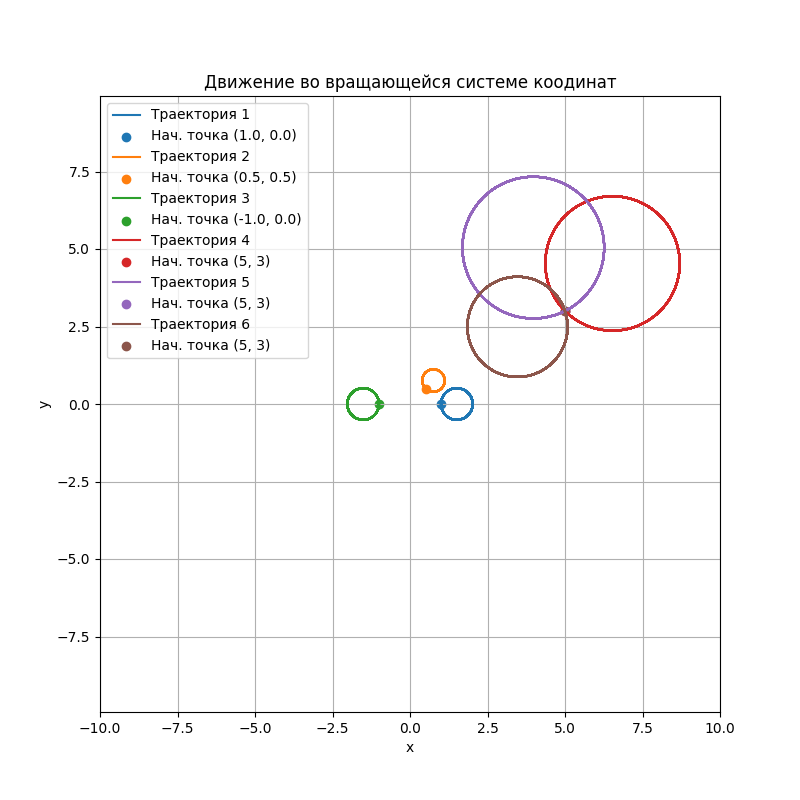
\includegraphics[height=0.8\textwidth]{imgs/1_78.png}  % Вставка изображения
	\caption{Траектории при \(\omega = 1, \phi = 78\) град.}  % Подпись к изображению
	\label{fig:1pi4}  % Метка для ссылки
\end{figure}

Увеличим  широту $\phi$ до 88 град и получим: 
\begin{figure}[h]  % Окружение для картинки
	\centering
	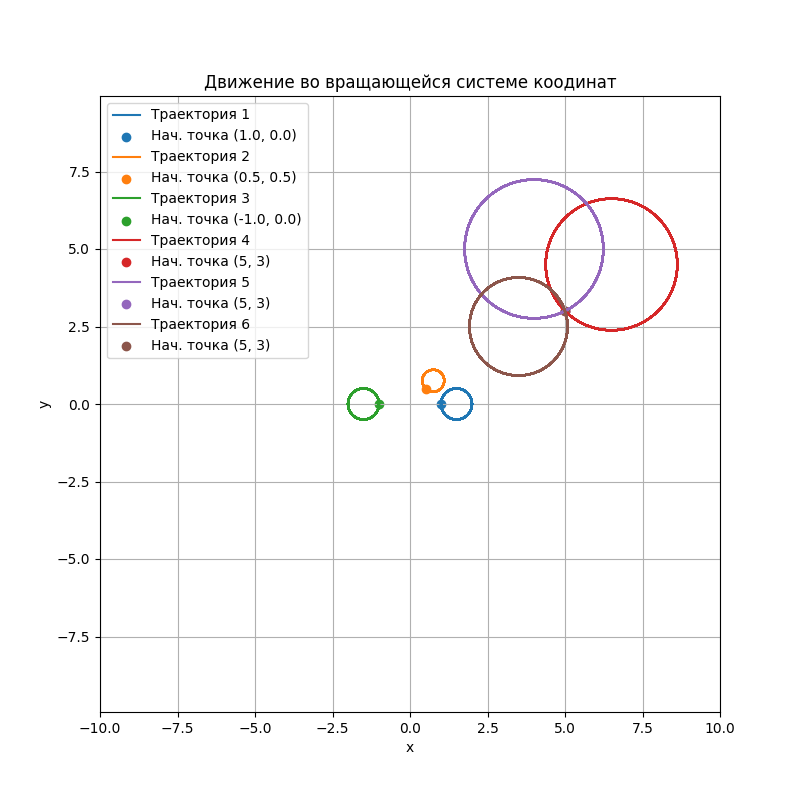
\includegraphics[height=0.8\textwidth]{imgs/1_88.png}  % Вставка изображения
	\caption{Траектории при \(\omega = 1, \phi = 88\) град.}  % Подпись к изображению
	\label{fig:1pi2.5}  % Метка для ссылки
\end{figure}

На рис. \ref{fig:1pi4} - \ref{fig:1pi2.5} видно, что при увеличении широты сила Кориолиса увеличивается, что влечёт увеличение влияния на относительную скорость, а следовательно, уменьшения радиусов описываемых траекторий.

Увеличим угловую скорость $\omega$ в 3 раза и также построим траектории при широтах 78 и 88 град.:
\begin{figure}[h]  % Окружение для картинки
	\centering
	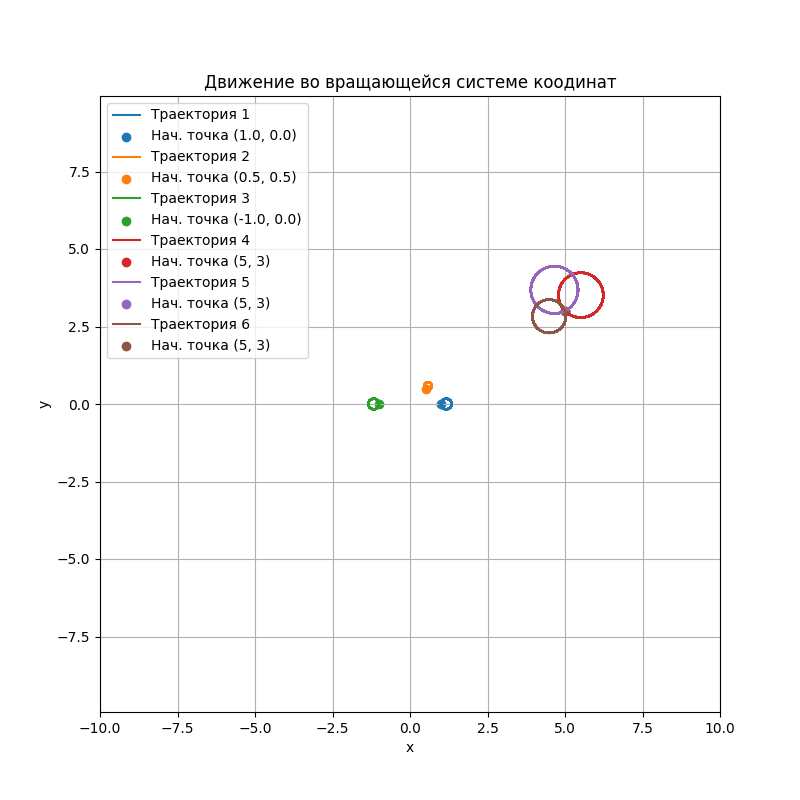
\includegraphics[height=0.7\textwidth]{imgs/3_78.png}  % Вставка изображения
	\caption{Траектории при \(\omega = 3, \phi = 78\) град.}  % Подпись к изображению
	\label{fig:10pi4}  % Метка для ссылки
\end{figure}


\begin{figure}[h]  % Окружение для картинки
	\centering
	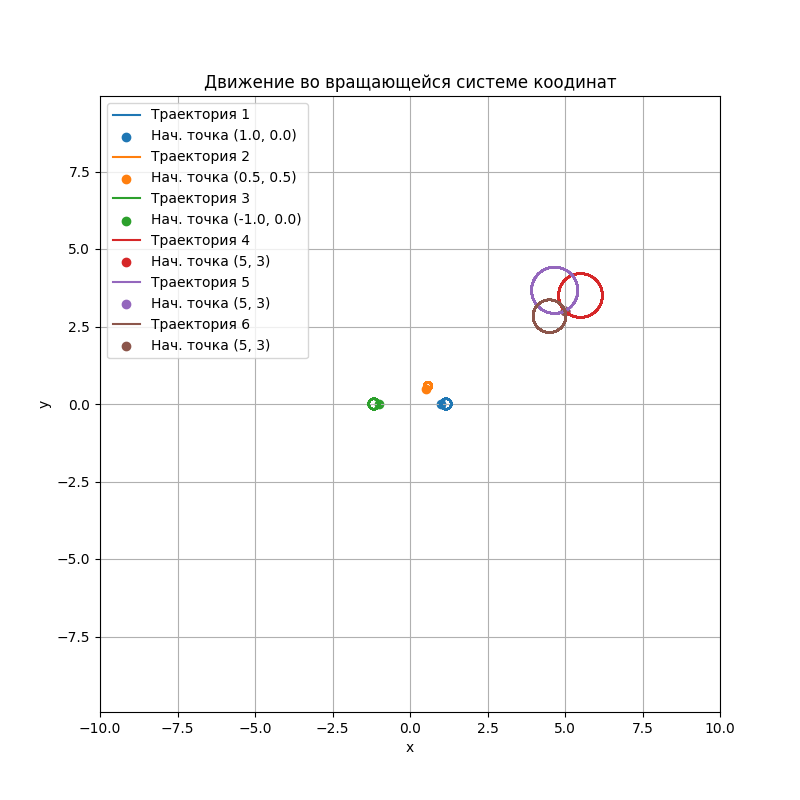
\includegraphics[height=0.7\textwidth]{imgs/3_88.png}  % Вставка изображения
	\caption{Траектории при \(\omega = 3, \phi = 88\) град.}  % Подпись к изображению
	\label{fig:10pi2.5}  % Метка для ссылки
\end{figure}
\newpage

Заметим (рис. \ref{fig:10pi4} - \ref{fig:10pi2.5}), что при увеличении угловой скорости, радиусы траекторий значительно уменьшились. Но при увеличении широты заметен эффект увеличения влияния силы Кориолиса.


